% !TeX root = ../main.tex

\section{Simulation Study}

\subsection{Data Simulation}

To test the CarHHMM with STFT, a sequence of 100 marine-animal dives were simulated. The coarse-scale observations $Y$ were set as the duration of each dive, and the fine-scale observations $Y^*$ were set as one dimensional acceleration readings simulated at 50 hertz. Specifically, the following procedure was followed: 

\begin{enumerate}
	\item 100 dive durations were simulated using an HMM generative model with the following parameters:
	
	\begin{align*}
		\Gamma &= \begin{pmatrix} 0.4 & 0.6 \\ 0.6 & 0.4 \end{pmatrix} \\
		% 
		&Y_t|X_t \sim Gamma \\
		\bbE(Y_t|X_t = 1) &= 15 s, \quad \bbE(Y_t|X_t = 2) = 60 s \\
		%
		\bbV(Y_t|X_t = 1) &= 25 s^2, \quad \bbV(Y_t|X_t = 2) = 100 s^2
	\end{align*}
	
	\item Once the dive durations were calculated, for each $t \in \{1, \ldots, 100\}$, dive $t$ was broken into $\lfloor Y_t/2 \rfloor$ 2-second segments (the end of the dive sequence was discarded). Further, each 2-second segment was assigned a behaviour according to a fine-scale Markov chain $X^*_t$, where $X^*_{t,t^*} \in \{1,2\}$ and $t^* \in \{1,101,201,\ldots,100*\lfloor Y_t/2 \rfloor + 1\}$. The parameters of the fine-scale behaviour Makov chain were set to be as follows:
	%
	$$\Gamma^{*(1)} = \begin{pmatrix} 0.25 & 0.75 \\ 0.75 & 025 \end{pmatrix} \qquad 	\Gamma^{*(2)} = \begin{pmatrix} 0.75 & 0.25 \\ 0.25 & 0.75 \end{pmatrix}$$
	%
	where $\Gamma^{*(1)}$ was used for dives where $X_t = 1$ and $\Gamma^{*(2)}$ was used for dives where $X_t = 2$
	
	\item For each 2-second segment, the Fourier modes $\hat{Y}^*_{t,t^*}$ were simulated using the following procedure. Note that the $n^{th}$ Fourier mode of $\hat{Y}^*_{t,t^*}$ is denoted as $\hat{Y}^{*(n)}_{t,t^*}$ :
	
	\begin{align*}
	\hat{Y}^{*(0)}_{t,1} &\sim \mathcal{N} \left(\mu = 1, \sigma^2 = 0.01 \right) & \\
	%
	\hat{Y}^{*(0)}_{t,t^*} &\sim \mathcal{N} \left(\mu = 0.9 Y^{*(0)}_{t,t^*-100} + 0.1, \sigma^2 = 0.01 \right), & t^* \in \{101,201,\ldots, 100*\lfloor Y_t/2 \rfloor + 1\} \\
	%
	\hat{Y}^{*(n)}_{t,t^*} &= a_{t,t^*}^{(n)} i\sqrt{b^{(n)}_{t,t^*}}, & n \in \{1,\ldots,49\} \\\\
	%
	%
	a_{t,t^*}^{(n)} &\sim  \left\{\begin{array}{lr}
	-1 & w.p. \enspace 1/2 \\
	1  & w.p. \enspace 1/2
	\end{array}\right. \\
	%
	(b^{(n)}_{t,t^*}|X^*_{t,t^*}  = 1) &\sim Gamma(1/n^2, 1) & \\
	%
	(b^{(n)}_{t,t^*}|X^*_{t,t^*} = 2) &\sim  \left\{\begin{array}{lr}
	Gamma(1/n^2, 1) & \text{for } n \neq 2\\
	Gamma(100,1) & \text{for } n = 2
	\end{array}\right. & \\\\
	%
	%
	\hat{Y}^{*(50)}_{t,t^*} &= 0 & \\
	%
	\hat{Y}^{*(n)}_{t,t^*}  &= -\hat{Y}^{*(100-n)}_{t,t^*}, & \qquad n \in \{51,\ldots,99\}
	\end{align*}
	
	Finally, $Y^*_{t,t^*:t^*+99}$ is set using the inverse discrete fourier transform of $\hat{Y}^*_{t,t^*}$:
	
	$$Y^*_{t,t^*:t^*+99} = IDFT\left(\hat{Y}^*_{t,t^*}\right)$$
	
	This gives a strong periodic component to acceleration when the subdive state $X^*_{t,t^*}= 2$. There are several practical reasons behind this construction:

	\begin{enumerate}
		\item $\hat{Y}^*_{t,t^*}$ is anti-symetric about $\hat{Y}^{*(50)}_{t,t^*}$ so that its inverse fourier transform is real-valued.
		\item $\hat{Y}^{*(n)}_{t,t^*}$ decays like $1/n^2$ to facilitate continutity.
	\end{enumerate}
		
\end{enumerate}

Note that this process idoes not result in a continuous sequence $Y^*_t$ since the average values of consecutive 2-second segments jump. However, note that these average values are highly autocorrelated, so the jumps are not too severe. See figure (\ref{fig:sim_data}) for details. In addition, $Y^*_t$ has the following desirable properties:

\begin{enumerate}
	\item $Z^{*(1)}_{t,t^*+1} | Z^{*(1)}_{t,t^*} \sim \mathcal{N} \left(\mu = 0.9 Z^{*(1)}_{t,t^*} + 0.1, \sigma^2 = 0.01 \right)$
	\item $$Z^{*(2)}_{t,t^*} \sim \left\{\begin{array}{lr} 
	\text{Gamma}(\sum_{n=1}^{\tilde{w}} \frac{1}{n^2},1) & \text{for } X^*_{t,t^*} = 1 \\
	\text{Gamma}(20 + \sum_{n=2}^{\tilde{w}} \frac{1}{n^2},1) & \text{for } X^*_{t,t^*} = 2
	\end{array}\right. $$
\end{enumerate}

So we can directly compare the results of the CarHHMM with the ground truth.

\begin{figure}[!ht]
	\centering
	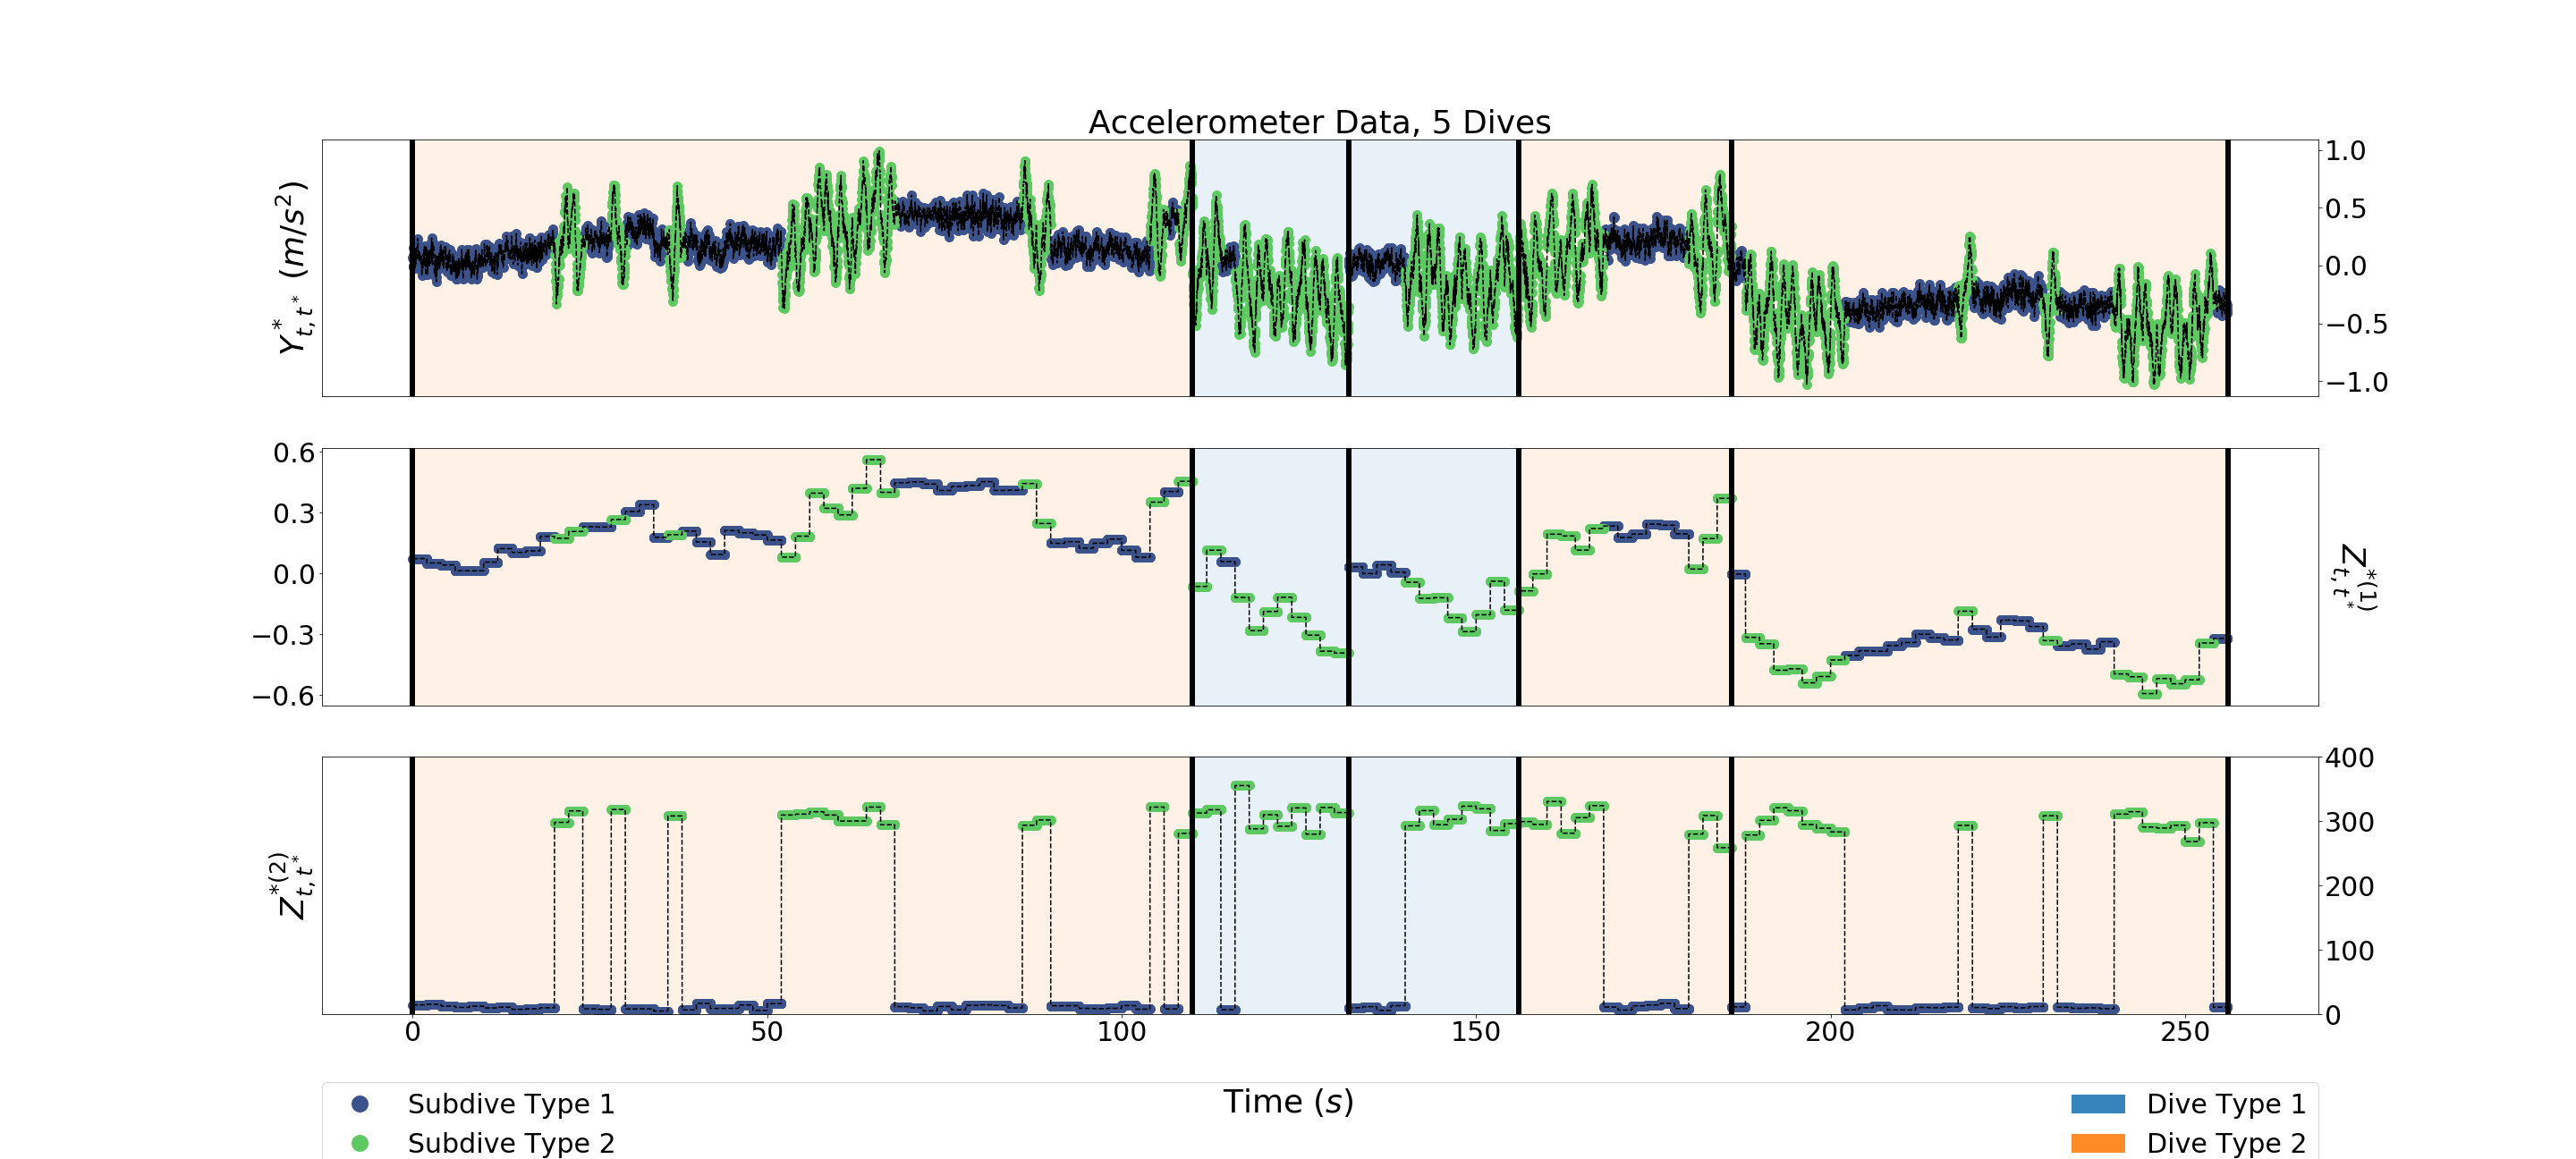
\includegraphics[width=5in]{../Plots/sim_data.png}
	\caption{Simulated Acceleration Data.}
	\label{fig:sim_data}
\end{figure}
I still need to put in the actually results from the simulation study- I had to rethink how to do the simulation in the first place since enforcing continuity was REALLY hard to do in a principled way. 

\iffalse
\subsection{Model Misspecification}

There are two ways to simulate the fourier modes of the acceleration vector $\bfA_{s,t}$:

\begin{enumerate}
	\item $$\bbE_1\left(\bfA_{s,t} | \bfA_{s-1,t}, X^*_{s,t}\right) = \phi \bfA_{s-1,t} + (1-\phi) \mu_{X^*_{s,t}} $$
	
	\item $$\bbE_2(\bfA_{s,t} | \bfA_{s-1,t}, X^*_{s,t}, X^*_{s-1,t}) = \left\{\begin{array}{lr}
	\phi \bfA_{s-1,t} + (1-\phi) \mu_{X^*_{s,t}} & \text{for } X^*_{s,t} = X^*_{s-1,t}\\
	\mu_{X^*_{s,t}} & \text{for } X^*_{s,t} \neq X^*_{s-1,t}
	\end{array}\right\}$$
\end{enumerate}

\subsubsection{$\bbE_1$}

First, look at $\bbE_1$. This comes with an issue in that when $X^*_{s,t}$ changes values, it will take a while for the process to ``converge" long-run mean $\mu_{X^*_{s,t}}$. In particular, if the behavioral process $X^*$ had been in state 1 for a while and then switches to state 2 for a while, then:

\begin{align*}
	\bbE_1\left(\bfA_{s+1,t}|X^*_{s:s+1,t} = 2, X^*_{s,t} = 1\right) &=  \phi \mu_1 + (1-\phi) \mu_2 \\
	%
	\bbE_1\left(\bfA_{s+2,t}|X^*_{s:s+2,t} = 2, X^*_{s,t} = 1\right) &= \phi\left( \phi \mu_1 + (1-\phi) \mu_2\right) + (1-\phi)\mu_2 \\
	&= \phi^2 \mu_1 + (1-\phi^2) \mu_2\\
	%
	\bbE_1\left(\bfA_{s+n,t}|X^*_{s:s+n,t} = 2, X^*_{s,t} = 1\right) &=  \phi^n \mu_1 + (1-\phi^n) \mu_2 \\
\end{align*}

So, if using $\bbE_1$, there is an assumption that the fourier modes of the acceleration vector $\bfA$ linearly ``converge" to the new value $\mu_i$ from $\mu_j$ when $X^*_{s,t}$ changes from $i$ to $j$. An example of this can be seen in figure (\ref{fig:FOVEDBA}).

 \begin{figure}[h!]
 	\centering
 	\includegraphics[height=3in]{../Code/test.png}
 	\caption{The FoVeDBA of simulated data using $\bbE_1$. Note that the FoVeDBA approaches $\approx$ 300 in state 2 from $\approx$ 10 in state 1 with roughly linear convergence.}
 	\label{fig:FOVEDBA}
 \end{figure}
 
 Note that if the generative model is correlated, but the inference model isn't, then quick jumps between states 1 and 2 can be missed because the chain never ``converges" to the new mean $\mu_i$, as shown in figure (\ref{fig:STATE}).
 
\begin{figure}[h!]
	\centering
	\includegraphics[height=3in]{../Code/test2.png}
	\caption{The probability of being in each behavioral state $X^*_{s,t}$ as estimated by the HHMM. The colors represent the true behavioral state.}
	\label{fig:STATE}
\end{figure}
 
 \subsubsection{$\bbE_2$}
 
Clearly, the model has issues decodeing the behavioral state when the model is misspecified. Therefore, if the true generative process does not have correlation when jumping between states, then it is better to use $\bbE_2$:

$$\bbE_2(\bfA_{s,t} | \bfA_{s-1,t}, X^*_{s,t}, X^*_{s-1,t}) = \left\{\begin{array}{lr}
\phi \bfA_{s-1,t} + (1-\phi) \mu_{X^*_{s,t}} & \text{for } X^*_{s,t} = X^*_{s-1,t}\\
\mu_{X^*_{s,t}} & \text{for } X^*_{s,t} \neq X^*_{s-1,t}
\end{array}\right\}$$

This fixes the issue of having to ``converge" to the new value of $\mu_i$ when jumping to state $i$. However, note that $\bbE_2$ depends upon both $X^*_{s,t}$ and $X^*_{s-1,t}$. This breaks the assumption in the forward algorithm that $\bfA_{s,t}$ depends only on $X^*_{s,t}$. One way to deal with this issues is to introduce a new hidden state $Z^*_{s,t} = (X^*_{s-1,t},X^*_{s,t})$. This fixes the issue, but now $Z^*_{s,t}$ can take one of $s^2$ values instead of $s$. This grows the state space of our model and can make inference harder.
 
 \fi
 
%Figure (\ref{fig:smoothing}) also shows the calculated ODBA as a function of time for one a specific dive. The acceleration exhibits sinusoidal behavior at several points in time which cannot be modeled using HMMs straightforwardly. As a result, the data was split into two-second intervals (100 data points each), and each interval was summarized by the Fourier transform of the ODBA and the velocity at the \textit{end} of the time interval. Velocity was taken at the end of the time interval because the behavior of the whale during the time interval has no impact on the velocity of the whale at the beginning of the time interval. Because velocity is highly correlated with the average acceleration within an interval, the mean was subtracted out of each ODBA time series before the Fourier transform was taken. To reduce the dimension of the ODBA Fourier transform, Fourier coefficients corresponding to frequencies less than or equal to 5 hertz were summed and frequencies above 5 hertz were ignored. One nice property of this process is that it reduces the number of data points by a factor of 100, which drastically speeds up parameter estimation. The optimal length of the time interval over which to take the Fourier transform is a tuning parameter that is difficult to find. An ideal time interval should be long enough give useful Fourier coefficients, but short enough to preserve as much information about the vertical velocity of the animal as possible.

%\subsection{Lag Plot}

%In order to find the appropriate HMM to model whale behavior, a lag plot was made for both velocity and the ODBA fourier sum. The results of doing so are shown in figure (\ref{fig:lag}). Unfortunately, the number of behavioral states is not clear from the lag plot, but it is clear that the velocity exhibits a large degree of autocorrelation. While the ODBA Fourier sum also exhibits some autocorrelation, the relationship is less strong, so autocorrelation was not incorporated in the ODBA Fourier sums emission distribution.